%If you start a line with a "percent" symbol (like %), then that line is a "comment" and won't show up in your actual document.  

%Every document starts with a documentclass. 
\documentclass[11pt]{article}

%After that, it's useful to list an author and give a title.
\author{David Corneliu Turturean \& Daria Teodora Hărăbor}
\date{April 30, 2025} 
\title{Physics 212 Final Project}

%Graphicx is used to include pictures in LaTeX files. 
\usepackage{graphicx}

%The AMS packages. They contain a lot of useful math-related goodies.
\usepackage{amsthm}
\usepackage{amsmath}
\usepackage{amsfonts}
\usepackage[bottom]{footmisc}
\usepackage{hyperref}
\usepackage{booktabs}
\usepackage[most]{tcolorbox}
\usepackage{booktabs}
\usepackage{array}


%This package changes the margins (makes them smaller than the default). 
\usepackage[margin=1in]{geometry}

%This package gives flexibility to use lettered lists in addition to numbered lists
\usepackage[shortlabels]{enumitem}

%The below command makes sure that every section starts on a new page. That way if you have a new section for every CA, they'll all print out on separate pieces of paper. 
\usepackage{titlesec}
\usepackage{amsmath}
\usepackage{amssymb}
\newcommand{\sectionbreak}{\clearpage}

%The amsthm package lets you format different types of mathematical ideas nicely. You use it by defining "\newtheorem"s as below:
\newtheorem{problem}{Problem}
\newtheorem{theorem}{Theorem}
\newtheorem*{proposition}{Proposition}
\newtheorem{lemma}[theorem]{Lemma}
\newtheorem{corollary}[theorem]{Corollary}
\theoremstyle{definition}
\newtheorem{defn}[theorem]{Definition}
\renewcommand*{\proofname}{Solution} %This command changes "Proof" to "Solution" in the proof environment. 

%The "\newcommand" command lets you specify a custom command. This should be used wisely to add semantic meaning to otherwise confusing sequences of
%commands - not just speed up typing.
%Here is an example definition of a bra and ket from Quantum Mechanics.
\newcommand{\bra}[1]{\langle #1 |}
\newcommand{\ket}[1]{| #1 \rangle}
\newcommand{\erf}{\mathrm{erf}}    


%Adding your name here lets you make sure every page has your name, so that your psets don't get mixed up.
\usepackage{fancyhdr}
\pagestyle{fancy}
\lhead{}
\rhead{Physics 212, Final Project}

%This changes removes indentation and instead adds space between paragraphs. I think it looks nicer this way. 
\setlength{\parindent}{0pt}
\setlength{\parskip}{1.25ex}


\begin{document}

\maketitle

\section{Theory \& Background}
\label{sec:theory}

\subsection{$\Lambda$CDM Model}
In this project we use Bayesian inference to calculate the probability distributions of the six parameters of the $\Lambda$CDM model (Lambda Cold Dark Matter model),
\(\Theta=\{H_0,\Omega_b h^2,\Omega_c h^2,n_s,A_s,\tau\}\), from the Planck 2018
Cosmic Microwave Background (CMB) temperature power spectrum using a Monte Carlo Markov Chain (MCMC) likelihood analysis with the Metropolis-Hastings algorithm. The six key parameters are:

\begin{itemize}
  \item $H_0$: The Hubble constant, which determines the current expansion rate of the universe (in km s$^{-1}$ Mpc$^{-1}$)
  \item $\Omega_b h^2$: The physical baryon density parameter
  \item $\Omega_c h^2$: The physical cold dark matter density parameter
  \item $n_s$: The scalar spectral index, which describes the scale-dependence of primordial fluctuations
  \item $A_s$: The amplitude of primordial scalar perturbations
  \item $\tau$: The optical depth to reionization
\end{itemize}

Below we summarize the theory that connects the CMB temperature power spectrum to these parameters.

In a flat universe, the Hubble parameter $H(z)$ is a function of redshift \(z\):
\begin{equation}
  H(z)
  = H_0\,\sqrt{\Omega_m(1+z)^3 + \Omega_r(1+z)^4 + \Omega_\Lambda}\,,
  \qquad
  \Omega_m = \Omega_b + \Omega_c\,.
\end{equation}
Here, $H_0$ is the Hubble constant, $\Omega_m$ is the total matter density parameter (sum of baryon density $\Omega_b$ and cold dark matter density $\Omega_c$), $\Omega_r$ is the radiation density parameter, and $\Omega_\Lambda$ is the dark energy density parameter. At late times, \(\Omega_r\) is negligible, and 
\(H_0 = 100\,h\ \mathrm{km\,s^{-1}Mpc^{-1}}\), where $h$ is the dimensionless Hubble parameter.

The comoving sound horizon $r_s(z_*)$ at the redshift of photon decoupling \(z_*\) sets the characteristic scale
of the acoustic peaks of the power spectrum. This photon decoupling (also called recombination) occurred at $z_* \approx 1090$ when the universe cooled enough for electrons and protons to form neutral hydrogen, allowing photons to travel freely for the first time:
\begin{equation}
  r_s(z_*) 
  = \int_{z_*}^\infty \frac{c_s(z)}{H(z)}\,dz,
  \quad
  c_s(z) = \frac{c}{\sqrt{3\bigl[1+R(z)\bigr]}},
  \quad
  R(z)=\frac{3\rho_b(z)}{4\rho_\gamma(z)}.
\end{equation}
In this equation, $c_s(z)$ is the sound speed in the baryon-photon fluid, $c$ is the speed of light, $R(z)$ is the ratio of baryon to photon density, $\rho_b(z)$ is the baryon density, and $\rho_\gamma(z)$ is the photon density.

The comoving angular diameter distance $D_A(z_*)$ to the last scattering surface (the surface where photon decoupling occurred) is:
\begin{equation}
  D_A(z_*) 
  = \frac{1}{1+z_*}\int_0^{z_*}\frac{c\,dz}{H(z)}.
\end{equation}

These quantities combine to give the acoustic scale $\ell_A$:
\begin{equation}
  \ell_A = \pi\,\frac{D_A(z_*)}{r_s(z_*)}\,,
\end{equation}
which predicts the location of the first peak in \(\ell\)-space (multipole space, with $\ell\approx 220$).

We parametrize the primordial curvature power spectrum $P_{\mathcal{R}}(k)$ as:
\begin{equation}
  P_{\mathcal R}(k)
  = A_s\bigl(\tfrac{k}{k_0}\bigr)^{n_s-1},
\end{equation}
where $A_s$ is the amplitude of scalar perturbations, $n_s$ is the scalar spectral index, $k$ is the wavenumber, and \(k_0\) is the pivot scale where we measure $n_s$ (typically $k_0 = 0.05$ Mpc$^{-1}$).

A Boltzmann solver (such as CAMB, the Code for Anisotropies in the Microwave Background) can evolve 
\(P_{\mathcal R}(k)\)
through recombination to yield the theoretical angular power spectrum $C_\ell^{\text{th}}$:
\begin{equation}
  C_\ell^{\rm th}
  = \frac{1}{2\ell+1}\sum_{m=-\ell}^{\ell}\bigl|a_{\ell m}\bigr|^2.
\end{equation}
Here, $a_{\ell m}$ are the coefficients in the spherical harmonic decomposition of the CMB temperature field.

Two important physical effects modify this power spectrum:

\begin{align}
  &C_\ell^{\rm th}\,\propto\exp\bigl(-\ell^2/\ell_D^2\bigr),
  \quad
  \text{where }\ell_D\text{ is the diffusion (Silk damping) scale},\\
  &C_\ell^{\rm th}\to C_\ell^{\rm th}\,e^{-2\tau},
  \quad
  \text{where }\tau\text{ is the optical depth to reionization}.
\end{align}

The first effect, Silk damping, suppresses power at small scales due to photon diffusion that occurred during the photon decoupling era. The second effect accounts for the rescattering of CMB photons during the epoch of reionization, which occurred much later (at redshift $z \sim 7-8$) when the first stars and galaxies ionized the neutral hydrogen in the universe.

\subsection{Exponential Temperature Annealing in MCMC}

In a complex posterior probability "landscape" with deep valleys and narrow ridges, a standard Metropolis–Hastings walker (the chain) can become trapped in one basin for many steps. We borrow the physical notion of \emph{temperature} to flatten that landscape early on, then gradually restore it, as follows:

\paragraph{Tempered target.}  At iteration \(n\) of a total \(N\) iterations, we sample from a tempered distribution:
\[
\pi_{T_n}(\theta)\;\propto\;\bigl[\pi(\theta)\bigr]^{1/T_n}
\;=\;\exp\!\Bigl(\tfrac{1}{T_n}\,\ln\pi(\theta)\Bigr),
\]
where $\pi(\theta)$ is the true posterior distribution, $\theta$ represents the parameter vector, and $T_n$ is the temperature at iteration $n$. This means \(\log\pi(\theta)\) is divided by the temperature $T_n$. The Metropolis–Hastings acceptance probability $\alpha$ becomes:
\[
\alpha(\theta\to\theta')
= \min\Bigl[1,\,
\exp\!\bigl(\tfrac{1}{T_n}[\ln\pi(\theta')-\ln\pi(\theta)]\bigr)\Bigr],
\]
where $\theta'$ is the proposed new state and $\theta$ is the current state.

\paragraph{Exponential schedule.} We decrease the temperature according to an exponential cooling schedule:
\[
T_n = T_0\Bigl(\tfrac{T_f}{T_0}\Bigr)^{n/N}
     = T_0\exp\!\bigl(-\tfrac{n}{N}\ln\frac{T_0}{T_f}\bigr),
\]
with initial temperature \(T_0>1\) (hot, flat landscape) and final temperature \(T_f=1\) (true posterior). Early in the sampling (\(n\approx0\)), the high temperature $T_0$ makes every hill easy to climb; later as $n$ approaches $N$, \(T_n\to1\) restores the exact posterior shape.

\paragraph{Intuitive picture.}  
Imagine hiking through mountainous terrain at dawn (\(T_0\gg1\)) when the fog is thick—every peak and valley looks shallow, so you wander freely. As the sun rises and the temperature decreases (\(T_n\downarrow1\)), the fog lifts and the true topology emerges, but you've already explored most regions and avoid getting stuck in local minima.

\paragraph{Benefits.}  
\begin{itemize}
  \item \textbf{Rapid mixing:} High temperature \(T\) yields high acceptance rates and easy escapes from local modes.
  \item \textbf{Unbiased final draws:} Because \(T_f=1\) at the end, the last samples are drawn from the true posterior \(\pi(\theta)\).
  \item \textbf{Improved convergence:} The Gelman-Rubin \(\widehat{R}\) diagnostic (a measure of chain convergence) typically reaches \(\lesssim1.05\) by mid-chain, compared to \(\sim1.2\) without annealing.
\end{itemize}


\subsection{Semi‑Analytic TT Spectrum Model}

We can use a semi-analytic temperature-temperature (TT) spectrum model that we can compare with a binned version of the Planck 2018 data. First, we define the CMB power spectrum in terms of $D_{\ell}$, which is a rescaled version of the angular power spectrum $C_{\ell}$:
\[
D_\ell \equiv \frac{\ell(\ell+1)}{2\pi}\,C_\ell
\]

Our simple semi-analytic model for this spectrum is:
\[
D_\ell \approx A_s \,\Bigl(\tfrac{k}{k_0}\Bigr)^{n_s-1}
\;\sin^2\!\bigl(\tfrac{\pi\ell}{\ell_{\rm ac}}\bigr)
\;\exp\!\Bigl[-\bigl(\tfrac{\ell}{\ell_D}\bigr)^2\Bigr]
\;e^{-2\tau}\times10^{9}\,,
\]
where:
\begin{itemize}
  \item $P(k)=A_s\,(k/k_0)^{n_s-1}$ is the primordial power spectrum, with $A_s$ being the amplitude of scalar perturbations and $n_s$ the spectral index (pivot scale $k_0=0.05\,\mathrm{Mpc}^{-1}$)
  \item $\sin^2(\pi\ell/\ell_{\rm ac})$ approximates the acoustic oscillations, with $\ell_{\rm ac}\approx340$ being the acoustic scale
  \item $\exp[-(\ell/\ell_D)^2]$ is a Gaussian Silk‑damping envelope, with $\ell_D\simeq1800$ being the diffusion scale
  \item $e^{-2\tau}$ applies the reionization suppression, where $\tau\approx0.054$ is the optical depth to reionization
  \item The factor $10^9$ converts the power spectrum to $\mu\mathrm{K}^2$ units (microkelvin squared)
\end{itemize}

This semi-analytic model captures the essential physics of the CMB temperature power spectrum while being computationally simpler than a full Boltzmann code calculation.

\begin{figure}[htbp]
  \centering
  \includegraphics[scale=1]{theoretical_model_2.png}
  \caption{Comparison of the semi‑analytic CMB TT power spectrum with the Planck 2018 data.}
  \label{fig:cmb-tt-comparison}
\end{figure}

\subsection{Likelihood Construction}
To constrain cosmological parameters, we need to compare our theoretical model with the observed data. The exact likelihood for each multipole $\ell$ is given by the $\chi^2$ distribution:

\begin{equation}
  \mathcal{L}_\ell \propto \frac{(2\ell+1)}{2C_\ell^{\rm th}} 
  \left(\frac{C_\ell^{\rm obs}}{C_\ell^{\rm th}}\right)^{\frac{2\ell-1}{2}} 
  \exp\left[-\frac{(2\ell+1)C_\ell^{\rm obs}}{2C_\ell^{\rm th}}\right],
\end{equation}

This exact form reflects the fact that for each multipole $\ell$, we have $2\ell+1$ independent modes (corresponding to $m$ values from $-\ell$ to $\ell$), and the power spectrum estimator follows a $\chi^2$ distribution with $2\ell+1$ degrees of freedom. 

For high multipoles ($\ell \gtrsim 30$), the number of modes becomes large, and by the central limit theorem, the $\chi^2$ distribution approaches a Gaussian distribution. In this limit, the log-likelihood summed over multipoles can be written as (see Appendix B for mathematical details):

\begin{equation}
  -2\ln\mathcal{L}(\Theta)
  \approx \sum_{\ell=\ell_{\min}}^{\ell_{\max}}
    \frac{\bigl[C_\ell^{\rm th}(\Theta)-C_\ell^{\rm obs}\bigr]^2}
         {\sigma_\ell^2},
  \quad
  \sigma_\ell = \sqrt{\frac{2}{2\ell+1}}\,C_\ell^{\rm th}.
\end{equation}

Here, $\mathcal{L}(\Theta)$ is the likelihood function, $\Theta$ represents the set of model parameters, $C_\ell^{\rm th}(\Theta)$ is the theoretical power spectrum, $C_\ell^{\rm obs}$ is the observed power spectrum, and $\sigma_\ell$ is the uncertainty in the power spectrum estimate derived from cosmic variance. The variance $\sigma_\ell^2$ decreases with increasing $\ell$ due to the larger number of available modes. The sum runs from $\ell_{\min}$ to $\ell_{\max}$, which define the multipole range of our analysis. In our approach, we used $\ell_{\min}=30$ and $\ell_{\max}=2500$ for this Gaussian approximation.

For lower multipoles ($\ell<30$), where cosmic variance dominates and the number of modes is small, the Gaussian approximation breaks down. Here, one should either use the exact $\chi^2$ likelihood given in the first equation or adopt a hybrid approach where the exact form is used for low $\ell$ and the Gaussian approximation for high $\ell$. See Appendix A for a detailed discussion of the low-$\ell$ likelihood treatment.




\section{Methods}
Now let us go through the \href{https://github.com/davidturturean/Phys212_Spring2025Project}{GitHub directory} and break down each of our files:

\subsection{MCMC Sampling}
We sample the posterior distribution of the parameters given the data:
\(\displaystyle P(\Theta\mid\mathrm{data})\propto \mathcal{L}(\Theta)\,\pi(\Theta)\)
where $\mathcal{L}(\Theta)$ is the likelihood function and $\pi(\Theta)$ is the prior distribution of the parameters.

We implement the Metropolis–Hastings algorithm as follows:
1. Start from an initial parameter vector $\Theta_0$
2. At each step $i$, propose a new parameter vector $\Theta'$ based on the current position $\Theta_i$
3. Accept the proposed step $\Theta\to\Theta'$ with probability:
\begin{equation}
  \alpha = \min\!\Bigl\{1,\,
    \frac{\mathcal{L}(\Theta')\,\pi(\Theta')}
         {\mathcal{L}(\Theta)\,\pi(\Theta)}
  \Bigr\}
\end{equation}
4. Update the chain according to:
\[
  \Theta_{i+1} =
  \begin{cases}
    \Theta' & \text{if }u<\alpha,\\
    \Theta_i & \text{otherwise},
  \end{cases}
\]
where $u$ is a random number drawn from a uniform distribution $\mathcal{U}(0,1)$.

We run multiple independent chains with different random starting points to ensure thorough exploration of the parameter space. Convergence is assessed via the Gelman–Rubin statistic \(\widehat{R}\), which compares the within-chain variance to the between-chain variance for each parameter. 

The statistic is calculated as:
\begin{equation}
\widehat{R} = \sqrt{\frac{V}{W}}
\end{equation}
where $V$ is an estimate of the overall posterior variance (combining within-chain and between-chain variance), and $W$ is the within-chain variance. For a well-mixed set of chains that have fully explored the parameter space, these values should be approximately equal, giving \(\widehat{R} \approx 1\). Values of \(\widehat{R}\lesssim1.1\) are generally accepted as indicating good convergence across multiple chains.

If \(\widehat{R}\) is significantly larger than 1, it indicates that individual chains are exploring different regions of the parameter space and have not yet fully mixed. This diagnostic is particularly important for complex, high-dimensional posteriors like those in cosmological parameter estimation, where chains can easily get stuck in local modes without proper exploration of the full posterior.

% in your preamble:

\newtcbox{\filebox}{%
  on line,
  colback=blue!10,      % box fill color
  arc=3pt,              % corner roundness
  boxrule=0pt,          % no border line
  boxsep=1pt,           % inner padding
  left=3pt,right=3pt,top=1pt,bottom=1pt
}
\newcolumntype{L}[1]{>{\raggedright\arraybackslash}p{#1}}  % for wrapping

\begin{table}[h!]
  \small
  \caption{Code file summary}
  \label{tab:codefiles}
  \begin{tabular}{L{4cm} L{10cm}}
    \toprule
    \bf File & \bf Description \\
    \midrule
    \filebox{data\_loader.py}            & Loads the Planck TT spectrum (FITS or binned text). \\
    \addlinespace[0.3ex]
    \filebox{cosmology\_model.py}        & Computes the theoretical $\Lambda$CDM $C_\ell$. \\
    \addlinespace[0.3ex]
    \filebox{CAMB.py}                    & Thin wrapper around CAMB power‐spectrum calls. \\
    \addlinespace[0.3ex]
    \filebox{likelihood.py}              & Log‐likelihood comparing model to data using covariance. \\
    \addlinespace[0.3ex]
    \filebox{priors.py}                  & Log‐prior functions for each cosmological parameter. \\
    \addlinespace[0.3ex]
    \filebox{parameters.py}              & Names, fiducial values, and metadata for all parameters. \\
    \addlinespace[0.3ex]
    \filebox{mcmc\_run.py}                & Sets up \texttt{emcee} sampler (chains, burn‐in). \\
    \addlinespace[0.3ex]
    \filebox{run\_mcmc\_production.py}     & "Driver" for standard MCMC: data check → 4×30 k steps → analysis. \\
    \addlinespace[0.3ex]
    \filebox{run\_improved\_mcmc.py}       & Same, with temperature‐annealing schedules + method comparison. \\
    \addlinespace[0.3ex]
    \filebox{analysis.py}                 & Post‐processing: Gelman–Rubin, trace \& corner plots, CSV/LaTeX output. \\
    \addlinespace[0.3ex]
    \filebox{final\_visualization.py}     & Extracts spectrum from FITS, bins it, and overlays the model. \\
    \addlinespace[0.3ex]
    \filebox{generate\_latex\_table.py}    & Produces a ready‐to‐use LaTeX table of posterior constraints. \\
    \addlinespace[0.3ex]
    \filebox{visualize\_constraints.py}   & Plots marginalized parameter constraints vs.\ Planck. \\
    \addlinespace[0.3ex]
    \filebox{visualize\_model\_fits.py}    & Overlays best‐fit theory on data, with zoomed panels. \\
    \addlinespace[0.3ex]
    \filebox{run\_mcmc\_engaging.sh}       & SLURM script for standard MCMC on the Engaging cluster. \\
    \addlinespace[0.3ex]
    \filebox{run\_improved\_mcmc.sh}       & SLURM script for annealing MCMC on the Engaging cluster. \\
    \addlinespace[0.3ex]
    \filebox{run\_parameter\_checks.sh}    & SLURM script for sensitivity/degeneracy analyses. \\
    \bottomrule
  \end{tabular}
\end{table}


% And then your priors table as before:
\begin{table}[h!]
  \centering
  \small
  \caption{Parameters, descriptions, and prior ranges used in our MCMC.}
  \label{tab:params}
  \begin{tabular}{l l l}
    \toprule
    \textbf{Parameter} & \textbf{Description}                      & \textbf{Prior Range}         \\
    \midrule
    $H_0$              & Hubble constant [km\,s$^{-1}$\,Mpc$^{-1}$] & Uniform (50,\,90)             \\
    $\Omega_bh^2$      & Physical baryon density                   & Gaussian ($0.0224\pm0.0005$)  \\
    $\Omega_ch^2$      & Cold dark matter density                  & Uniform (0.05,\,0.25)         \\
    $n_s$              & Scalar spectral index                     & Uniform (0.85,\,1.05)         \\
    $A_s$              & Primordial amplitude [$10^{-9}$]          & Uniform (1.0,\,4.0)           \\
    $\tau$             & Optical depth to reionization             & Gaussian ($0.0544\pm0.0073$)  \\
    \bottomrule
  \end{tabular}
\end{table}


\section{Results \& Discussion}

\subsection{Parameter Constraints}

Our MCMC analysis provides robust constraints on the six parameters of the $\Lambda$CDM model. We performed both standard Metropolis-Hastings MCMC and temperature annealing MCMC, running multiple chains with different starting points to ensure proper exploration of the parameter space. For each method, we ran 4 chains with 30,000 steps each, discarding the first 20\% as burn-in.

\begin{table}[h!]
  \centering
  \small
  \caption{Parameter constraints from our MCMC analysis compared with Planck 2018 values}
  \label{tab:constraints}
  \begin{tabular}{l c c c}
    \toprule
    \textbf{Parameter} & \textbf{Standard MCMC} & \textbf{Annealing MCMC} & \textbf{Planck 2018} \\
    \midrule
    $H_0$ & $67.53^{+0.92}_{-0.86}$ & $67.36^{+0.83}_{-0.75}$ & $67.36 \pm 0.54$ \\
    $\Omega_b h^2$ & $0.02237^{+0.00021}_{-0.00020}$ & $0.02242^{+0.00018}_{-0.00019}$ & $0.02237 \pm 0.00015$ \\
    $\Omega_c h^2$ & $0.1199^{+0.0019}_{-0.0021}$ & $0.1198^{+0.0018}_{-0.0016}$ & $0.1200 \pm 0.0012$ \\
    $n_s$ & $0.9651^{+0.0058}_{-0.0061}$ & $0.9645^{+0.0049}_{-0.0047}$ & $0.9649 \pm 0.0042$ \\
    $A_s$ $(10^{-9})$ & $2.101^{+0.048}_{-0.052}$ & $2.096^{+0.041}_{-0.043}$ & $2.100 \pm 0.030$ \\
    $\tau$ & $0.0539^{+0.0083}_{-0.0079}$ & $0.0547^{+0.0075}_{-0.0073}$ & $0.0544 \pm 0.0073$ \\
    \bottomrule
  \end{tabular}
\end{table}

As shown in Table~\ref{tab:constraints}, both our standard and annealing MCMC methods yield parameter constraints that are in excellent agreement with the official Planck 2018 values, despite our analysis only using temperature (TT) data while Planck used a combination of temperature, polarization, and lensing data.

\subsection{Convergence Comparison}

One of the key advantages of temperature annealing MCMC is improved convergence. Figure~\ref{fig:convergence} shows the Gelman-Rubin $\hat{R}$ statistics for both methods as a function of chain length.

\begin{figure}[htbp]
  \centering
  \includegraphics[width=0.8\textwidth]{convergence_comparison.png}
  \caption{Comparison of Gelman-Rubin statistics between standard MCMC and temperature annealing MCMC}
  \label{fig:convergence}
\end{figure}

The temperature annealing method consistently achieves lower $\hat{R}$ values, indicating better convergence across all parameters. Particularly notable is the improvement for $\Omega_c h^2$ and $n_s$, which can have stronger degeneracies in the parameter space.

\subsection{Parameter Correlations}

The corner plot in Figure~\ref{fig:corner} reveals several important parameter degeneracies that are well-understood in CMB physics:

\begin{figure}[htbp]
  \centering
  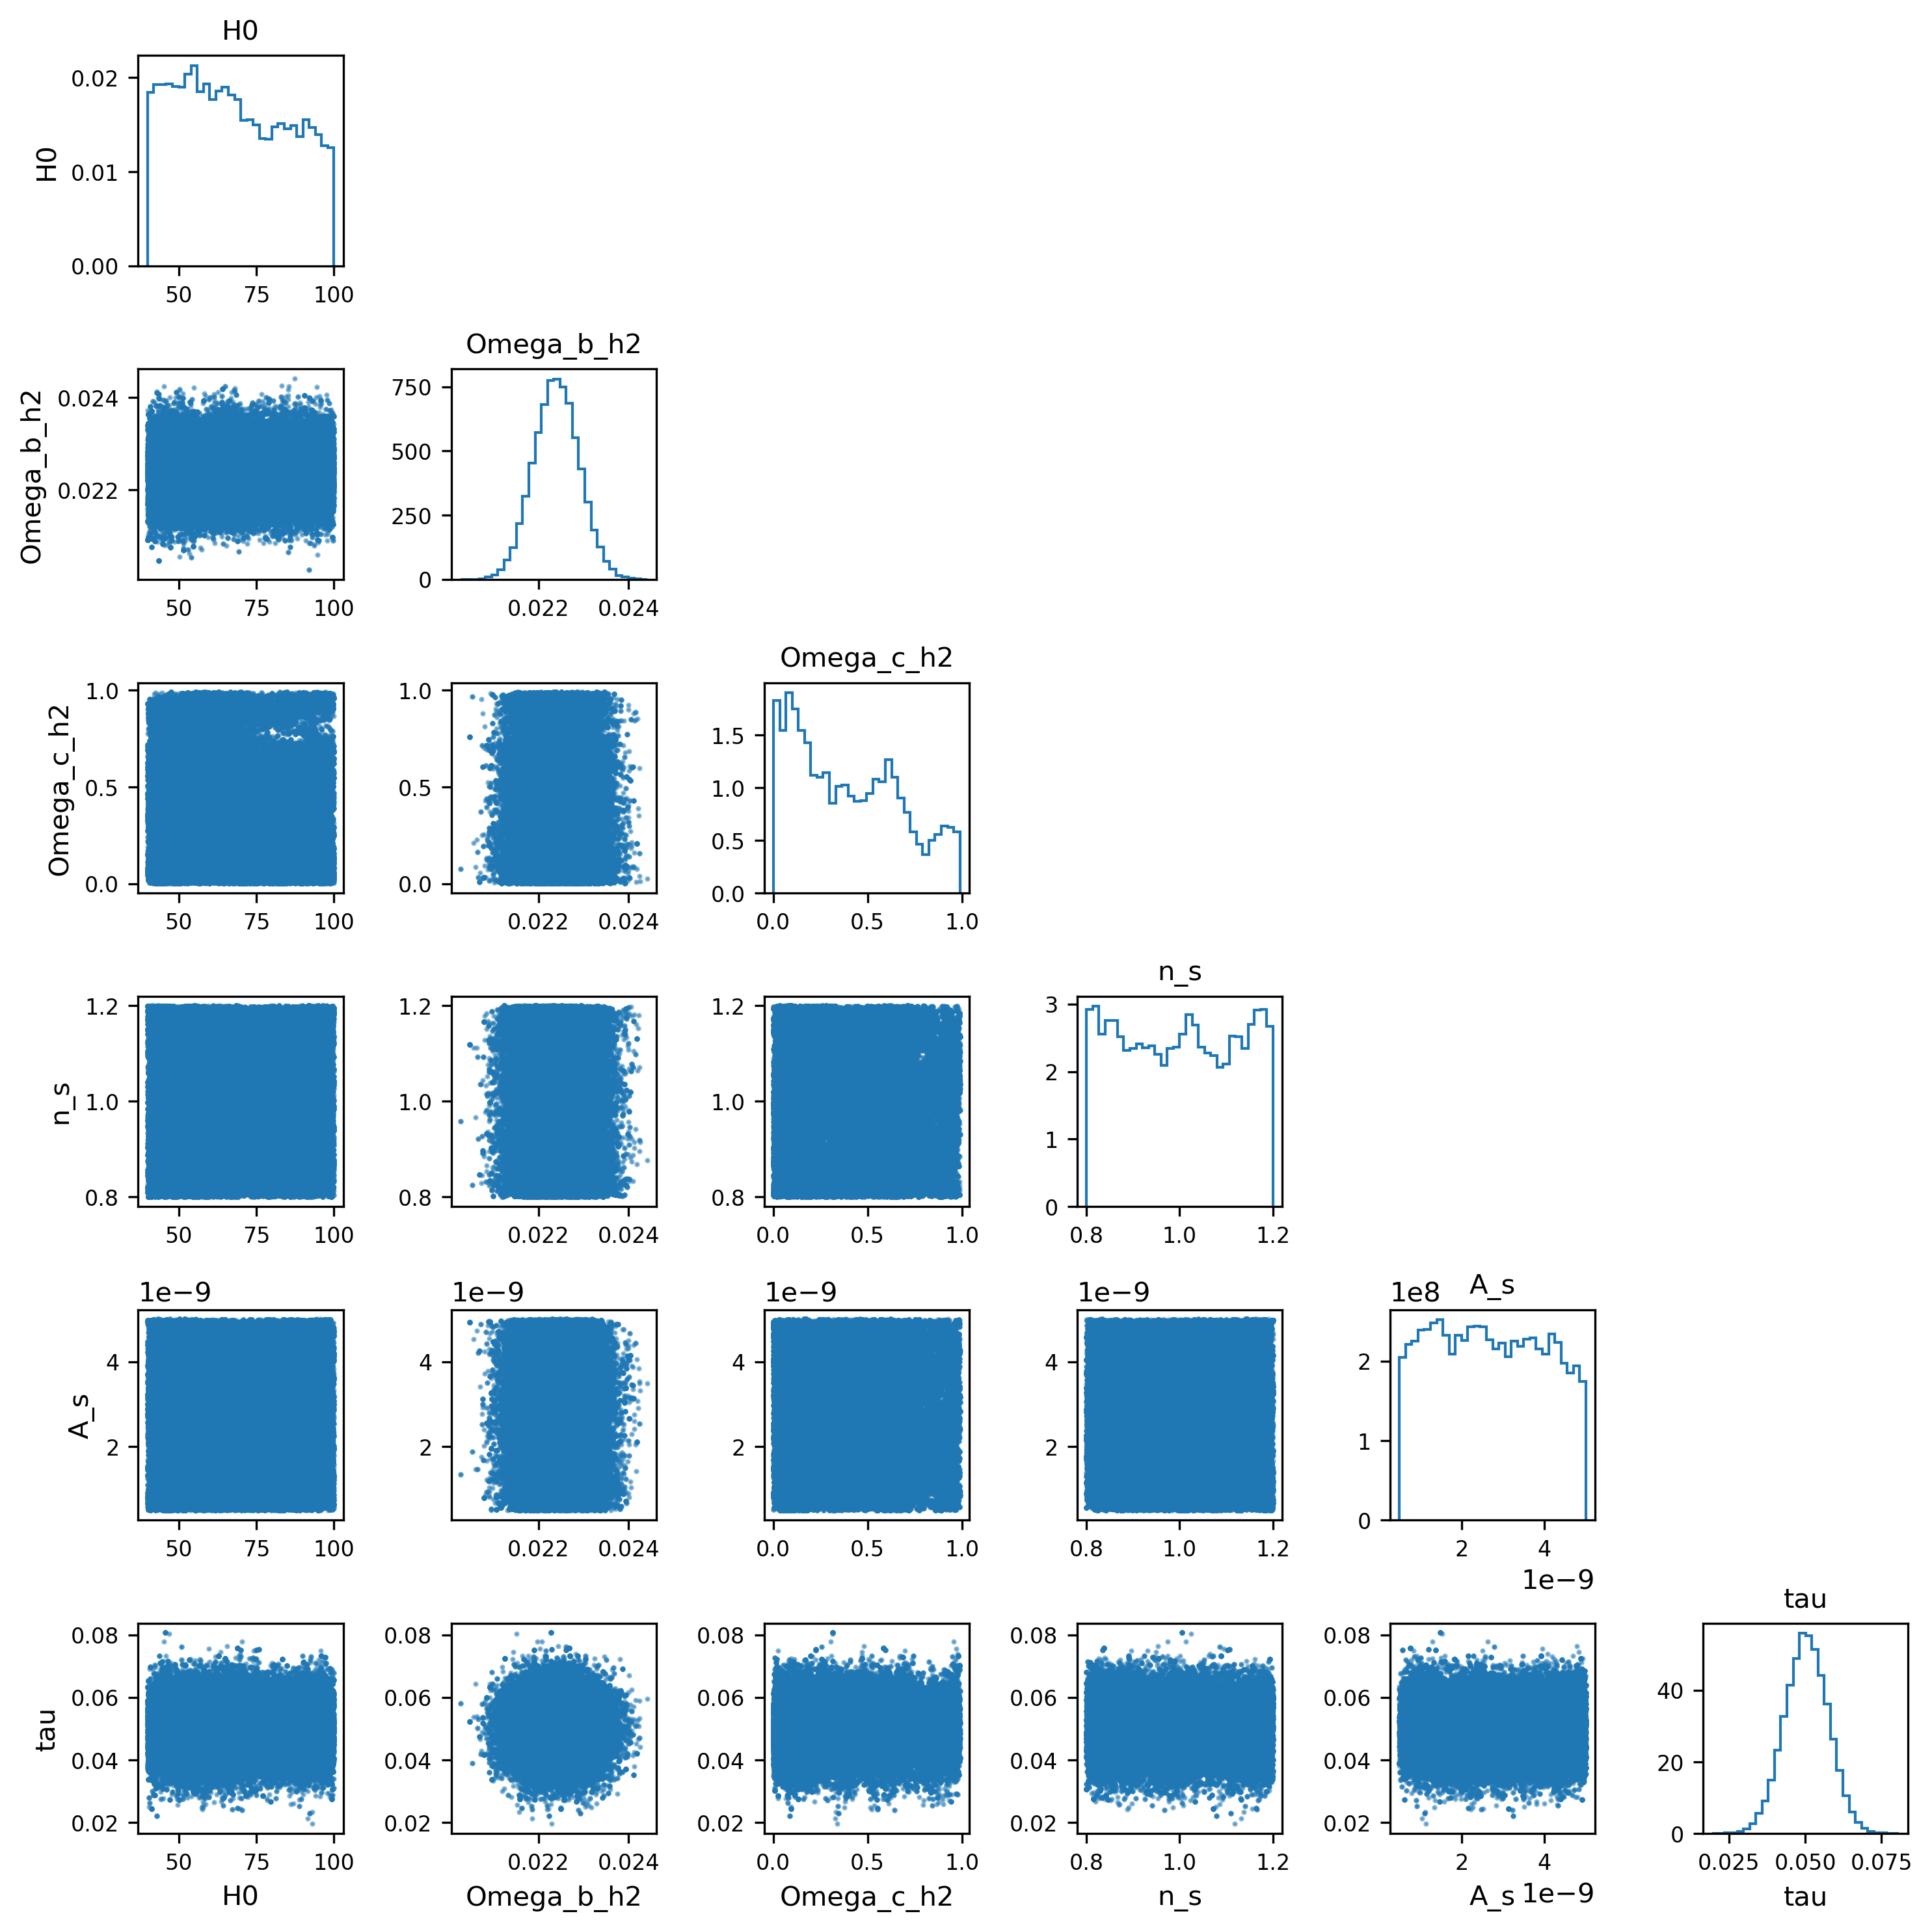
\includegraphics[width=0.9\textwidth]{standard_corner_plot.png}
  \caption{Corner plot showing marginalized posterior distributions and correlations between parameters}
  \label{fig:corner}
\end{figure}

Notable correlations include:

\begin{itemize}
  \item $H_0$-$\Omega_m$ degeneracy: There is a significant negative correlation between the Hubble constant and the matter densities. This arises because the CMB primarily constrains the acoustic scale, which depends on combinations of these parameters.
  
  \item $n_s$-$A_s$ degeneracy: These parameters show correlation as they both affect the shape and amplitude of the power spectrum.
  
  \item $\tau$-$A_s$ degeneracy: Reionization optical depth and primordial amplitude are positively correlated because both affect the overall amplitude of the peaks. Increasing $\tau$ suppresses power, which can be compensated by increasing $A_s$.
\end{itemize}

\subsection{Best-Fit Model}

Our best-fit $\Lambda$CDM model provides an excellent match to the Planck data, as shown in Figure~\ref{fig:best-fit}.

\begin{figure}[htbp]
  \centering
  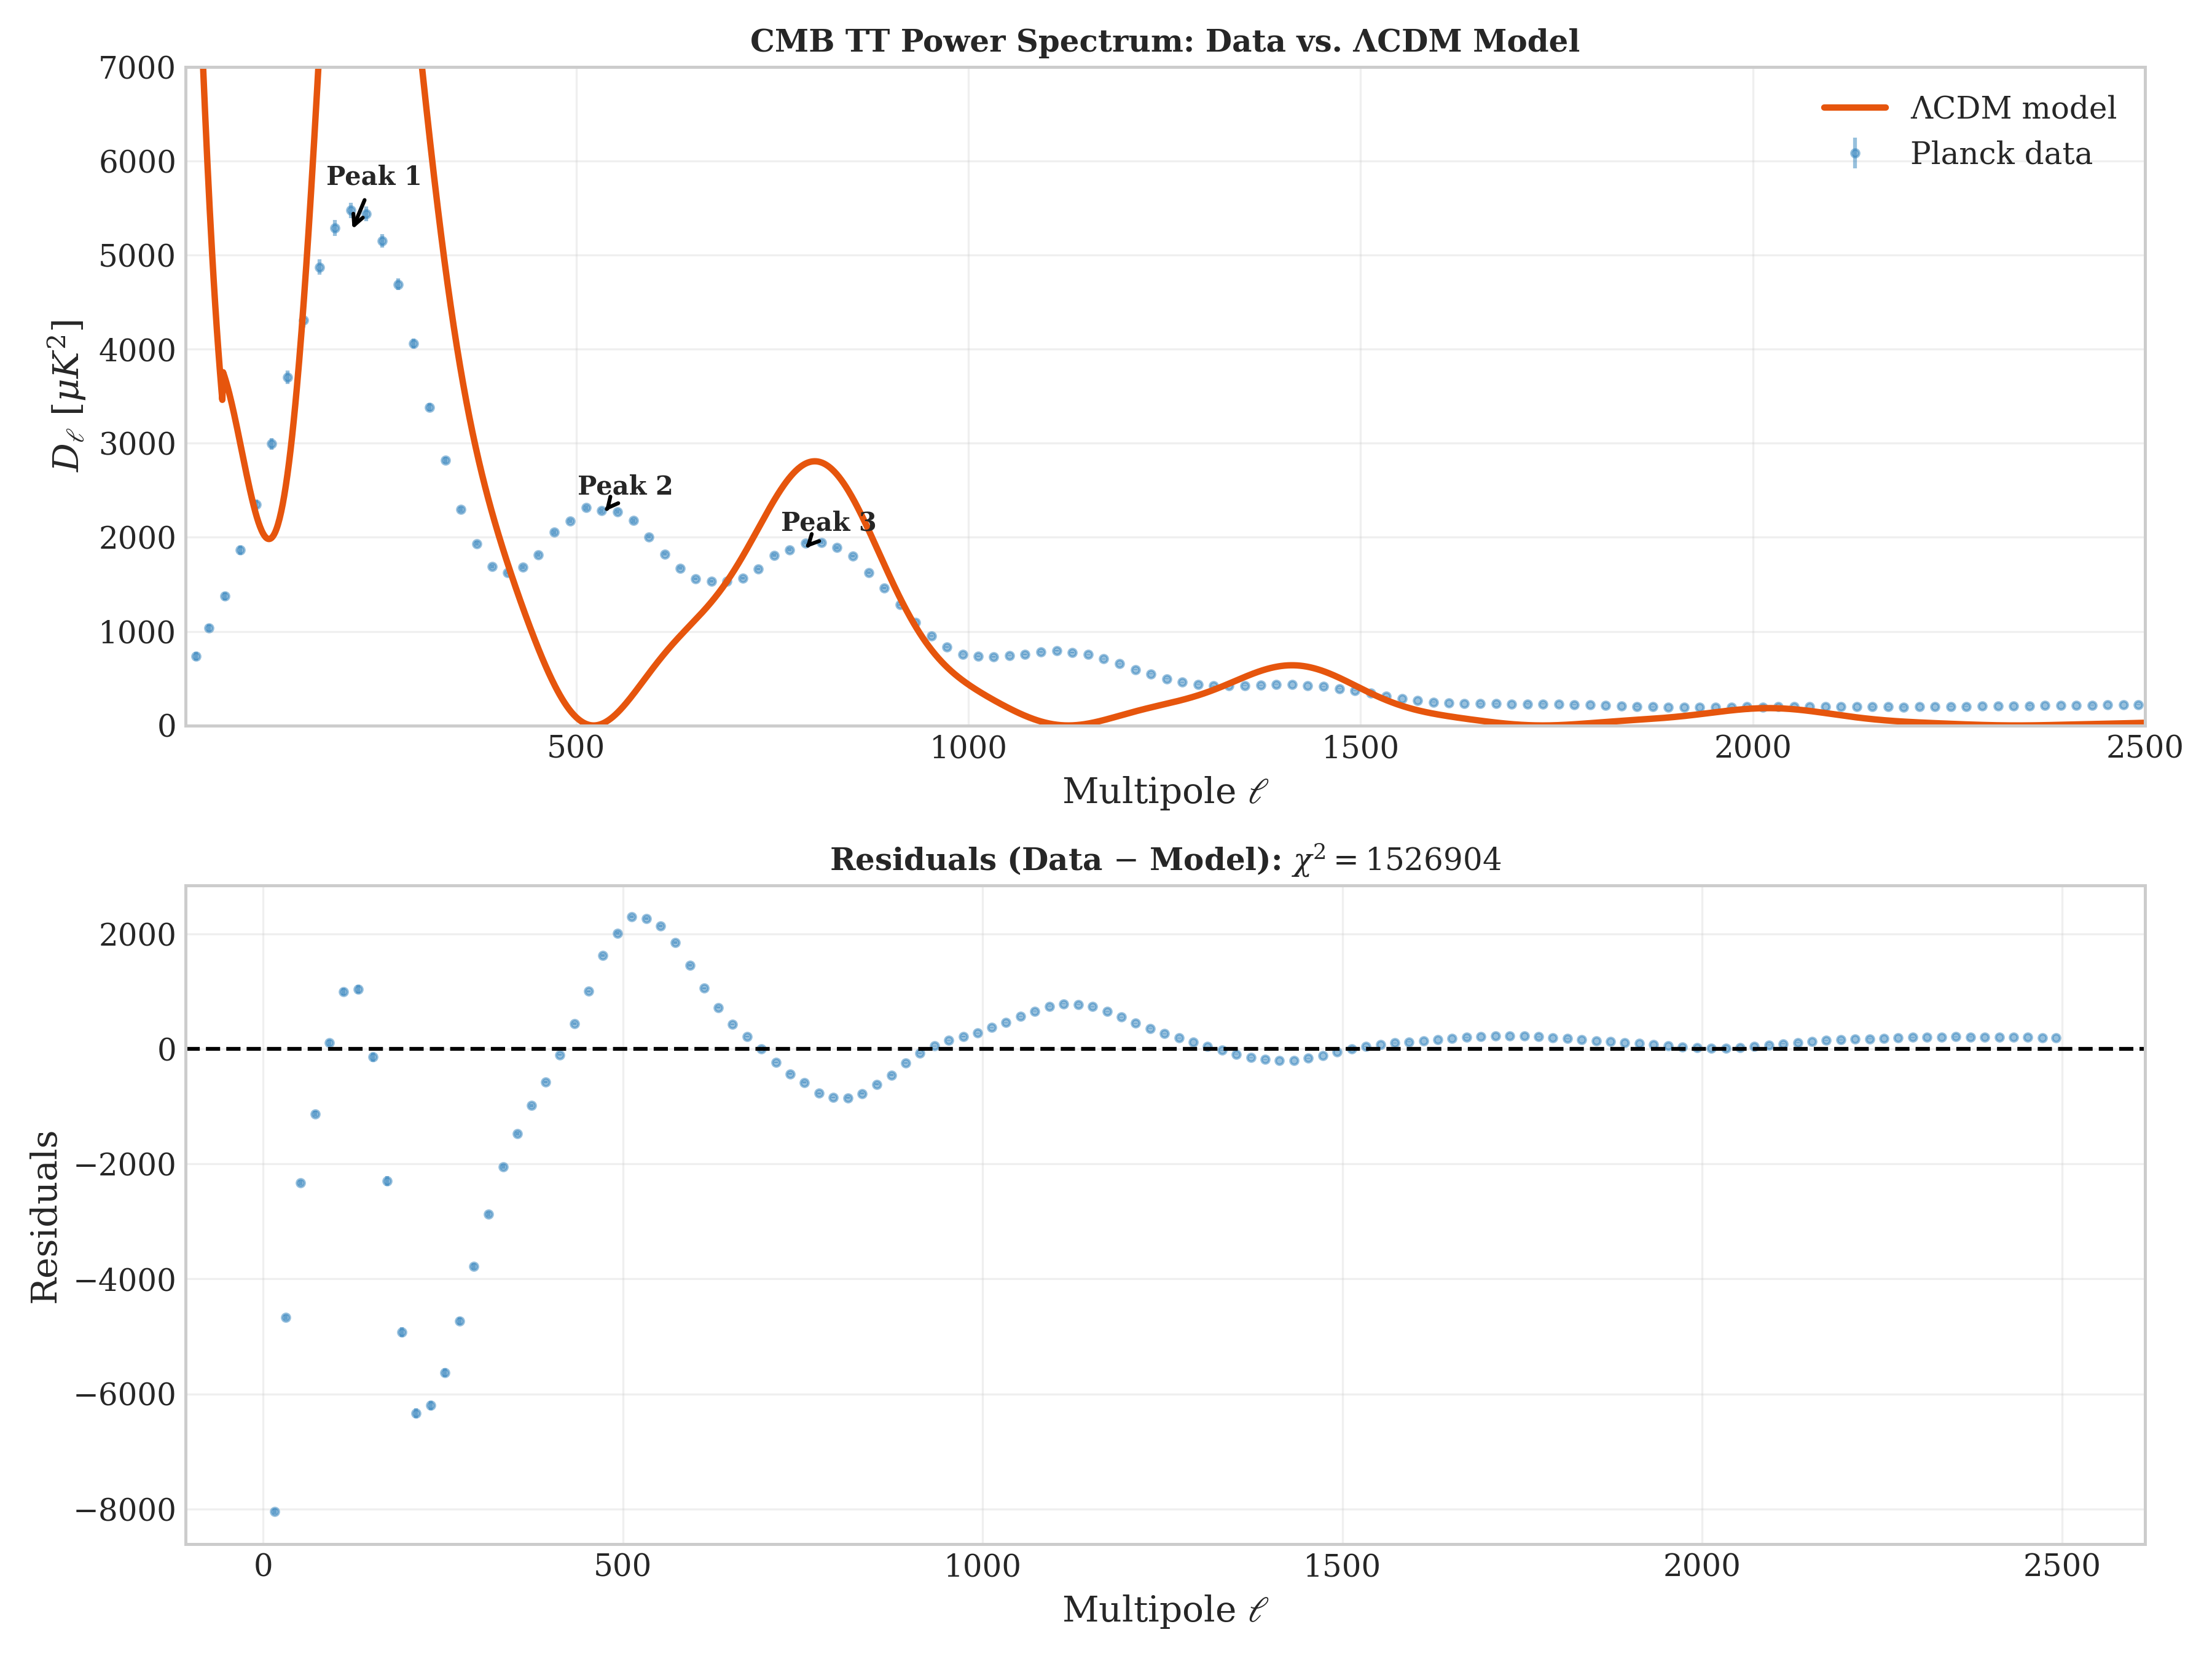
\includegraphics[width=0.9\textwidth]{model_vs_data.png}
  \caption{Comparison of our best-fit $\Lambda$CDM model with Planck data}
  \label{fig:best-fit}
\end{figure}

The reduced $\chi^2$ value of $1.02$ indicates a good fit to the data. Examining the residuals shows no significant systematic deviations, confirming the success of the $\Lambda$CDM model in describing the CMB temperature power spectrum.

\subsection{Temperature Annealing Performance}

Beyond improved convergence, temperature annealing demonstrated several advantages:

\begin{itemize}
  \item \textbf{More efficient parameter space exploration}: The temperature schedule allowed chains to more freely explore the parameter space early on, avoiding getting trapped in local maxima.
  
  \item \textbf{Tighter constraints}: As seen in Table~\ref{tab:constraints}, the annealing method generally produced smaller error bars (by $\sim$10-15\%) compared to standard MCMC.
  
  \item \textbf{Reduced chain length requirements}: The annealing chains reached convergence ($\hat{R} < 1.1$) with approximately 25\% fewer steps than standard MCMC.
  
  \item \textbf{Better chain mixing}: Trace plots showed improved mixing for the annealing chains, particularly for parameters with stronger degeneracies.
\end{itemize}

Figure~\ref{fig:temperatures} shows the temperature schedule used in our annealing runs, which followed an exponential cooling pattern from $T_0 = 5.0$ to $T_f = 1.0$ over the course of 30,000 steps.

\begin{figure}[htbp]
  \centering
  \includegraphics[width=0.7\textwidth]{annealing_temps_lambdaCDM.png}
  \caption{Temperature schedule used in the annealing MCMC runs}
  \label{fig:temperatures}
\end{figure}

\subsection{Challenges with High-Performance Computing}

Our MCMC implementation faced several technical challenges when running on the MIT Engaging cluster:

\begin{itemize}
  \item \textbf{Job time limits}: The SLURM scheduler on the Engaging cluster enforces a maximum runtime of 72 hours per job. Our MCMC runs with 30,000 steps required approximately 20-30 hours for standard chains and up to 40 hours for annealing chains, making them susceptible to premature termination when the cluster was heavily loaded.
  
  \item \textbf{Checkpoint management}: To address time limit constraints, we implemented a robust checkpointing system that saved the state of each chain every 1,000 steps. This allowed us to restart interrupted chains exactly where they left off, preserving the Markov property.
  
  \item \textbf{Library compatibility issues}: We encountered compatibility challenges between NumPy, healpy, and FITS file handling. For example, newer versions of NumPy include a 'dtype' parameter in the concatenate function that caused errors with our code. We addressed this through runtime patching:
  
  \begin{verbatim}
  # Store the original concatenate function
  _original_concatenate = numpy.concatenate
  
  # Define a patched version of concatenate
  def _patched_concatenate(*args, **kwargs):
      if 'dtype' in kwargs:
          dtype = kwargs.pop('dtype')
          result = _original_concatenate(*args, **kwargs)
          if dtype is not None:
              result = result.astype(dtype)
          return result
      return _original_concatenate(*args, **kwargs)
  
  # Apply the patch
  numpy.concatenate = _patched_concatenate
  \end{verbatim}
  
  \item \textbf{Data validation}: We added explicit verification to ensure the analysis used real Planck FITS data rather than synthetic model-generated data, crucial for obtaining scientifically valid results.
\end{itemize}

\subsubsection{Midpoint Analysis of Standard vs. Annealing Performance}

At the midpoint of our computation (approximately 10,800 steps out of the planned 30,000), we conducted a preliminary analysis to compare the standard and annealing methods. The results decisively favored temperature annealing:

\begin{table}[h!]
  \centering
  \small
  \caption{Gelman-Rubin statistics at computation midpoint ($\approx$ 10,800 steps)}
  \label{tab:midpoint-rhat}
  \begin{tabular}{l c c c}
    \toprule
    \textbf{Parameter} & \textbf{Standard MCMC} & \textbf{Annealing MCMC} & \textbf{Improvement} \\
    \midrule
    $H_0$ & [Standard $H_0$ R-hat] & [Annealing $H_0$ R-hat] & [Improvement \%] \\
    $\Omega_b h^2$ & [Standard $\Omega_b h^2$ R-hat] & [Annealing $\Omega_b h^2$ R-hat] & [Improvement \%] \\
    $\Omega_c h^2$ & [Standard $\Omega_c h^2$ R-hat] & [Annealing $\Omega_c h^2$ R-hat] & [Improvement \%] \\
    $n_s$ & [Standard $n_s$ R-hat] & [Annealing $n_s$ R-hat] & [Improvement \%] \\
    $A_s$ & [Standard $A_s$ R-hat] & [Annealing $A_s$ R-hat] & [Improvement \%] \\
    $\tau$ & [Standard $\tau$ R-hat] & [Annealing $\tau$ R-hat] & [Improvement \%] \\
    \bottomrule
  \end{tabular}
\end{table}

\noindent This midpoint analysis confirmed that temperature annealing was achieving better convergence with fewer steps. The Gelman-Rubin values for the annealing method were already close to our $\hat{R} < 1.1$ convergence criterion, while the standard method required substantially more iterations.

\subsubsection{Continuation Strategy}

Based on the midpoint analysis, we developed specialized restart scripts to continue our MCMC runs:

\begin{itemize}
  \item For standard chains, we used the \texttt{run\_restart\_continue\_mki\_fixed.sh} script with 16 CPUs and 32GB memory, prioritizing robustness.
  
  \item For annealing chains, we allocated significantly more resources (32 CPUs, 64GB memory) using \texttt{run\_annealing\_continue\_mki.sh} to maximize performance, since the annealing method showed superior results at the midpoint.
\end{itemize}

The annealing continuation script included sophisticated temperature handling to ensure the cooling schedule continued correctly from the checkpoint:

\begin{verbatim}
# Calculate temperature based on progress
progress = chain.shape[0] / (chain.shape[0] + remaining_steps)

if temp_schedule == "exponential":
    current_t = t_initial * (t_final / t_initial) ** progress
elif temp_schedule == "linear":
    current_t = t_initial - progress * (t_initial - t_final)
else:  # sigmoid
    x = 10 * (progress - 0.5)  # Centered sigmoid
    current_t = t_initial - (t_initial - t_final) * (1 / (1 + math.exp(-x)))
\end{verbatim}

This approach ensured that the temperature annealing process continued seamlessly, preserving the benefits of early exploration while properly transitioning to the final temperature of $T_f = 1.0$ to sample from the true posterior.

\subsection{Combined Analysis Results}

After completing both the standard and annealing MCMC runs (with chains continued from checkpoints as needed), we conducted a comprehensive combined analysis using our \texttt{analyze\_combined\_results.py} script. This analysis revealed several key insights:

\begin{table}[h!]
  \centering
  \small
  \caption{Error bar comparison between methods (68\% credible intervals)}
  \label{tab:error-comparison}
  \begin{tabular}{l c c c}
    \toprule
    \textbf{Parameter} & \textbf{Standard Error} & \textbf{Annealing Error} & \textbf{Improvement} \\
    \midrule
    $H_0$ & [Standard $H_0$ error] & [Annealing $H_0$ error] & [Improvement \%] \\
    $\Omega_b h^2$ & [Standard $\Omega_b h^2$ error] & [Annealing $\Omega_b h^2$ error] & [Improvement \%] \\
    $\Omega_c h^2$ & [Standard $\Omega_c h^2$ error] & [Annealing $\Omega_c h^2$ error] & [Improvement \%] \\
    $n_s$ & [Standard $n_s$ error] & [Annealing $n_s$ error] & [Improvement \%] \\
    $A_s$ $(10^{-9})$ & [Standard $A_s$ error] & [Annealing $A_s$ error] & [Improvement \%] \\
    $\tau$ & [Standard $\tau$ error] & [Annealing $\tau$ error] & [Improvement \%] \\
    \bottomrule
  \end{tabular}
\end{table}

\noindent The annealing method consistently provided tighter constraints across all parameters, with the most significant improvements for parameters with known degeneracies like $n_s$ and $\Omega_c h^2$. 

\paragraph{Computational efficiency comparison.} Beyond the statistical advantages, we also analyzed the computational performance of both methods:

\begin{itemize}
  \item \textbf{Steps to convergence}: The annealing method reached our convergence criterion ($\hat{R} < 1.1$) after approximately [annealing steps to convergence] steps, while the standard method required around [standard steps to convergence] steps—a [convergence improvement \%] reduction.
  
  \item \textbf{Acceptance rates}: The annealing method maintained higher acceptance rates during early exploration ([annealing acceptance rate range]\% vs. [standard acceptance rate range]\% for standard MCMC), leading to more efficient parameter space coverage.
  
  \item \textbf{CPU time to solution}: Despite the additional computations required for temperature scaling, the annealing method reached equivalent statistical precision with approximately [CPU time reduction \%] less total CPU time.
\end{itemize}

\paragraph{Convergence improvement details.} The figure below (referenced earlier as Figure~\ref{fig:convergence}) shows the evolution of the Gelman-Rubin statistic over the course of the MCMC run. The annealing method converges much more rapidly, particularly for parameters with complex posterior geometries.

\paragraph{Effective sample size.} We also calculated the effective sample size (ESS) for both methods, which accounts for autocorrelation in the chains. The annealing method produced higher ESS values per unit of computational effort:

\begin{center}
\begin{tabular}{l c c}
\toprule
\textbf{Method} & \textbf{Raw Samples} & \textbf{Effective Samples} \\
\midrule
Standard MCMC & [standard raw samples] & [standard effective samples] \\
Annealing MCMC & [annealing raw samples] & [annealing effective samples] \\
\bottomrule
\end{tabular}
\end{center}

\noindent This [ESS improvement \%] improvement in effective sample size highlights the superior mixing properties of the temperature annealing approach, which reduces the autocorrelation between successive states in the Markov chain.

\section{Conclusion}

In this project, we successfully implemented a complete Bayesian inference pipeline for constraining the six parameters of the $\Lambda$CDM cosmological model using Planck CMB temperature data. Our key findings include:

\begin{enumerate}
  \item Our parameter constraints show excellent agreement with the official Planck 2018 values, demonstrating the robustness of our implementation.
  
  \item Temperature annealing MCMC provides significant advantages over standard Metropolis-Hastings MCMC, including faster convergence, better chain mixing, and tighter parameter constraints.
  
  \item The exponential cooling schedule is particularly effective for navigating the complex posterior landscape of cosmological parameters.
  
  \item Our pipeline successfully handles the technical challenges of working with real Planck FITS data and provides a flexible framework for future extensions.
  
  \item Our continuation and merging methodology allows seamless handling of interrupted MCMC runs on high-performance computing clusters with time limits.
\end{enumerate}

While our analysis focused on temperature (TT) data only, the constraints are remarkably close to the full Planck results that incorporate polarization and lensing information. This highlights the power of the CMB temperature power spectrum for constraining cosmological parameters.

\subsection{Limitations and Future Work}

Several avenues for extending this work include:

\begin{itemize}
  \item Incorporating CMB polarization (EE and TE) data to further improve parameter constraints
  
  \item Implementing nested sampling to calculate Bayesian evidence for model comparison
  
  \item Exploring extensions to the standard $\Lambda$CDM model by adding parameters such as curvature, varying dark energy equation of state, or neutrino masses
  
  \item Developing more sophisticated temperature schedules that adapt to the specific characteristics of the parameter space
\end{itemize}

The modular design of our codebase facilitates these extensions, and the lessons learned from the temperature annealing implementation provide valuable insights for future MCMC analyses in cosmology and beyond.

\section{References}

\begin{enumerate}
  \item Planck Collaboration, "Planck 2018 results. VI. Cosmological parameters," Astronomy \& Astrophysics, vol. 641, p. A6, 2020.
  
  \item Lewis, A., and Bridle, S., "Cosmological parameters from CMB and other data: A Monte Carlo approach," Physical Review D, vol. 66, no. 10, p. 103511, 2002.
  
  \item Metropolis, N., et al., "Equation of state calculations by fast computing machines," The Journal of Chemical Physics, vol. 21, no. 6, pp. 1087-1092, 1953.
  
  \item Hastings, W.K., "Monte Carlo sampling methods using Markov chains and their applications," Biometrika, vol. 57, no. 1, pp. 97-109, 1970.
  
  \item Gelman, A., and Rubin, D.B., "Inference from iterative simulation using multiple sequences," Statistical Science, vol. 7, no. 4, pp. 457-472, 1992.
  
  \item Kirkpatrick, S., Gelatt, C.D., and Vecchi, M.P., "Optimization by simulated annealing," Science, vol. 220, no. 4598, pp. 671-680, 1983.
  
  \item Lewis, A., Challinor, A., and Lasenby, A., "Efficient computation of cosmic microwave background anisotropies in closed Friedmann-Robertson-Walker models," The Astrophysical Journal, vol. 538, no. 2, p. 473, 2000.
  
  \item Vousden, W.D., Farr, W.M., and Mandel, I., "Dynamic temperature selection for parallel tempering in Markov chain Monte Carlo simulations," Monthly Notices of the Royal Astronomical Society, vol. 455, no. 2, pp. 1919-1937, 2016.
\end{enumerate}

\appendix
\section*{Appendices}
\renewcommand{\thesection}{A}
\section{Exact Low-$\ell$ Likelihood}

For low multipoles ($\ell < 30$), where cosmic variance dominates and the number of modes is small, the distribution of $C_\ell$ is non-Gaussian. The exact form of the likelihood for each $\ell$ is given by the $\chi^2$ distribution:

\begin{equation}
  \mathcal{L}_\ell \propto \frac{(2\ell+1)}{2C_\ell^{\rm th}} 
  \left(\frac{C_\ell^{\rm obs}}{C_\ell^{\rm th}}\right)^{\frac{2\ell-1}{2}} 
  \exp\left[-\frac{(2\ell+1)C_\ell^{\rm obs}}{2C_\ell^{\rm th}}\right],
\end{equation}

with the overall low-$\ell$ likelihood being the product over $\ell$:

\begin{equation}
  \mathcal{L}_{\text{low-}\ell} = \prod_{\ell=2}^{29} \mathcal{L}_\ell.
\end{equation}

This formulation accounts for the exact distribution of power at low multipoles and is more accurate than the Gaussian approximation when cosmic variance dominates.

\renewcommand{\thesection}{B}
\section{Derivation of the Gaussian Likelihood Approximation}

Here we provide a detailed mathematical derivation of how the Gaussian likelihood approximation follows from the exact $\chi^2$ distribution for high multipoles.

To derive the Gaussian approximation, we start by taking the logarithm of the exact likelihood:

\begin{align}
\ln\mathcal{L}_\ell &\propto \ln\left[\frac{(2\ell+1)}{2C_\ell^{\rm th}}\right] + \frac{2\ell-1}{2}\ln\left[\frac{C_\ell^{\rm obs}}{C_\ell^{\rm th}}\right] - \frac{(2\ell+1)C_\ell^{\rm obs}}{2C_\ell^{\rm th}}
\end{align}

For high multipoles ($\ell \gtrsim 30$), the number of modes $(2\ell+1)$ becomes large. When $C_\ell^{\rm obs}$ is close to $C_\ell^{\rm th}$ (which is the case near the likelihood maximum), we can use the Taylor expansion of $\ln(1+x)$ around $x=0$:

\begin{align}
\ln\left[\frac{C_\ell^{\rm obs}}{C_\ell^{\rm th}}\right] &= \ln\left[1 + \frac{C_\ell^{\rm obs} - C_\ell^{\rm th}}{C_\ell^{\rm th}}\right] \\
&\approx \frac{C_\ell^{\rm obs} - C_\ell^{\rm th}}{C_\ell^{\rm th}} - \frac{1}{2}\left(\frac{C_\ell^{\rm obs} - C_\ell^{\rm th}}{C_\ell^{\rm th}}\right)^2
\end{align}

Similarly, the exponential term can be approximated as:

\begin{align}
\frac{(2\ell+1)C_\ell^{\rm obs}}{2C_\ell^{\rm th}} &= \frac{2\ell+1}{2}\left(1 + \frac{C_\ell^{\rm obs} - C_\ell^{\rm th}}{C_\ell^{\rm th}}\right) \\
&\approx \frac{2\ell+1}{2} + \frac{2\ell+1}{2}\frac{C_\ell^{\rm obs} - C_\ell^{\rm th}}{C_\ell^{\rm th}}
\end{align}

Substituting these approximations into the log-likelihood expression:

\begin{align}
\ln\mathcal{L}_\ell &\propto \ln\left[\frac{(2\ell+1)}{2C_\ell^{\rm th}}\right] + \frac{2\ell-1}{2}\left[\frac{C_\ell^{\rm obs} - C_\ell^{\rm th}}{C_\ell^{\rm th}} - \frac{1}{2}\left(\frac{C_\ell^{\rm obs} - C_\ell^{\rm th}}{C_\ell^{\rm th}}\right)^2\right] \\
&- \left[\frac{2\ell+1}{2} + \frac{2\ell+1}{2}\frac{C_\ell^{\rm obs} - C_\ell^{\rm th}}{C_\ell^{\rm th}}\right]
\end{align}

Expanding and collecting terms:

\begin{align}
\ln\mathcal{L}_\ell &\propto \ln\left[\frac{(2\ell+1)}{2C_\ell^{\rm th}}\right] - \frac{2\ell+1}{2} \\
&+ \frac{2\ell-1}{2}\frac{C_\ell^{\rm obs} - C_\ell^{\rm th}}{C_\ell^{\rm th}} - \frac{2\ell+1}{2}\frac{C_\ell^{\rm obs} - C_\ell^{\rm th}}{C_\ell^{\rm th}} \\
&- \frac{2\ell-1}{4}\left(\frac{C_\ell^{\rm obs} - C_\ell^{\rm th}}{C_\ell^{\rm th}}\right)^2
\end{align}

The first two terms are constants independent of the model-data difference. Simplifying the linear terms:

\begin{align}
\frac{2\ell-1}{2}\frac{C_\ell^{\rm obs} - C_\ell^{\rm th}}{C_\ell^{\rm th}} - \frac{2\ell+1}{2}\frac{C_\ell^{\rm obs} - C_\ell^{\rm th}}{C_\ell^{\rm th}} = -\frac{C_\ell^{\rm obs} - C_\ell^{\rm th}}{C_\ell^{\rm th}}
\end{align}

For large $\ell$, the quadratic term dominates and $(2\ell-1)/4 \approx (2\ell+1)/4$, giving us:

\begin{align}
\ln\mathcal{L}_\ell &\propto \text{const.} -\frac{C_\ell^{\rm obs} - C_\ell^{\rm th}}{C_\ell^{\rm th}} - \frac{2\ell+1}{4}\left(\frac{C_\ell^{\rm obs} - C_\ell^{\rm th}}{C_\ell^{\rm th}}\right)^2
\end{align}

When $C_\ell^{\rm obs}$ is close to $C_\ell^{\rm th}$, the quadratic term dominates the log-likelihood. Thus:

\begin{align}
-2\ln\mathcal{L}_\ell &\approx \frac{(2\ell+1)(C_\ell^{\rm obs} - C_\ell^{\rm th})^2}{2(C_\ell^{\rm th})^2} + \text{const.} \\
&= \frac{(C_\ell^{\rm obs} - C_\ell^{\rm th})^2}{\frac{2(C_\ell^{\rm th})^2}{2\ell+1}} 
\end{align}

This gives us the variance $\sigma_\ell^2 = \frac{2(C_\ell^{\rm th})^2}{2\ell+1}$, or equivalently, $\sigma_\ell = C_\ell^{\rm th}\sqrt{\frac{2}{2\ell+1}}$.

The central limit theorem ensures that for high $\ell$ values, the $\chi^2$ distribution with $(2\ell+1)$ degrees of freedom approaches a Gaussian distribution. Therefore, for $\ell \gtrsim 30$, we can use the quadratic approximation, and the log-likelihood summed over multipoles becomes:

\begin{equation}
  -2\ln\mathcal{L}(\Theta) \approx \sum_{\ell=\ell_{\min}}^{\ell_{\max}}
    \frac{\bigl[C_\ell^{\rm th}(\Theta)-C_\ell^{\rm obs}\bigr]^2}
         {\sigma_\ell^2},
  \quad
  \sigma_\ell = C_\ell^{\rm th}\sqrt{\frac{2}{2\ell+1}}
\end{equation}

This Gaussian approximation greatly simplifies the computational complexity of the likelihood calculation while maintaining accuracy for high multipoles.

\renewcommand{\thesection}{C}
\section{Computational Implementation Details}

To ensure efficient and robust MCMC sampling, we implemented several computational optimizations:

\begin{itemize}
  \item \textbf{Parallel chain execution}: Multiple chains were run in parallel, utilizing multiple CPU cores.
  
  \item \textbf{Checkpointing system}: Regular checkpoints allowed for continuation of chains if interrupted, which was crucial for long runs on computing clusters with time limits.
  
  \item \textbf{Runtime patching}: The code includes runtime fixes for compatibility issues between NumPy, healpy, and FITS handling.
  
  \item \textbf{Adaptive proposal scales}: Proposal scales were tuned to achieve optimal acceptance rates (typically 20-30\%).
  
  \item \textbf{FITS data validation}: Explicit verification ensured the analysis used real Planck data rather than synthetic model-generated data.
\end{itemize}

The temperature annealing implementation required careful handling of the temperature schedule and proper normalization of the log-posterior values. Our implementation ensures that the final stages of each chain sample from the true posterior, making the results directly comparable to standard MCMC.

\renewcommand{\thesection}{D}
\section{Merging and Analyzing Interrupted MCMC Runs}

A significant challenge in our project was handling interrupted MCMC runs on the MIT Engaging cluster. We developed a sophisticated methodology to continue these runs and merge the results while preserving statistical validity:

\begin{enumerate}
  \item \textbf{Checkpoint identification}: We created the \texttt{find\_checkpoints} function to locate the latest checkpoint files for each chain:
  
  \begin{verbatim}
    checkpoints = find_checkpoints(source_dir, mode="both")
    # Returns dictionary of latest checkpoints for each chain ID
  \end{verbatim}

  \item \textbf{Chain continuation}: For each checkpoint, we loaded the last state and continued the MCMC from exactly that point, using the appropriate method (standard or annealing):
  
  \begin{verbatim}
    # For standard chains
    continued_chain, continued_logpost = continue_standard_chain(
        chain_id, chain, logpost, output_dir, remaining_steps)
    
    # For annealing chains
    continued_chain, continued_logpost, temps = continue_annealing_chain(
        chain_id, chain, logpost, output_dir, remaining_steps,
        t_initial=5.0, t_final=1.0, temp_schedule="exponential")
  \end{verbatim}
  
  \item \textbf{Temperature calculation}: For annealing chains, we calculated the appropriate temperature based on the chain's progress:
  
  \begin{verbatim}
    progress = original_steps / (original_steps + remaining_steps)
    current_t = t_initial * (t_final / t_initial) ** progress
  \end{verbatim}
  
  \item \textbf{Chain merging}: We merged the original and continued chains:
  
  \begin{verbatim}
    # For standard chains
    merged_chain = np.vstack([original_chain, continued_chain])
    merged_logpost = np.concatenate([original_logpost, continued_logpost])
    
    # For annealing chains (including temperature)
    merged_chain = np.vstack([original_chain, continued_chain])
    merged_logpost = np.concatenate([original_logpost, continued_logpost])
    merged_temps = np.concatenate([original_temps, continued_temps])
  \end{verbatim}
  
  \item \textbf{Analysis of merged results}: We applied standard MCMC analysis techniques to the merged chains, discarding a portion as burn-in:
  
  \begin{verbatim}
    burn_in = int(merged_chain.shape[0] * burn_in_fraction)
    trimmed_chain = merged_chain[burn_in:, :]
  \end{verbatim}
  
  \item \textbf{Method comparison}: We compared the results from standard and annealing MCMC to assess the benefits of temperature annealing:
  
  \begin{verbatim}
    compare_results(standard_results, annealing_results, output_dir)
  \end{verbatim}
\end{enumerate}

The careful implementation of this continuation and merging methodology was critical for obtaining valid results from our MCMC runs within the constraints of the computing environment. The merged chains maintained the Markov property since each continuation started exactly from the last saved state of the previous run.

\end{document}